\subsection{\textit{HELLO}}
\label{sec:hello}

	O projeto HELLO (\textit{Handheld English Language Learning Organization}) integra os benefícios
	providos pela Realidade Aumentada, computação ubíqua e móvel com o objetivo de auxiliar na
	aprendizagem da língua inglesa~\cite{tsung}. Esse projeto utiliza a tecnologia denominada de
	\textit{m-learning (Mobile Learning)} para que os alunos tenham acesso a informação independente
	do local físico que eles estejam, flexibilizando e potencializando a aprendizagem. Seu conceito
	de~\textit{u-learning (Ubiquitous Learning)}, visa a possibilidade do usuário ser inserido em um
	ambiente onde ele tenha as informações de forma acessível e transparente, com o propósito de
	flexibilizar e tornar contínuo o processo de aprendizagem. Desta maneira, o usuário obtém
	vantagens providas pela~\textit{ubicomp}, tais como: acessibilidade, interatividade e sensibilidade
	ao contexto.
	
	O funcionamento do projeto HELLO é divido em subsistema servidor e um utilitário denominado
	\textit{u-Tools}. A aplicação servidor fica responsável pelo armazenamento das informações, tais
	como: materiais didáticos, aulas, banco de dados, provas, dentre outros. A \textit{u-Tools} foi
	desenvolvida para a plataforma utilizada pelos \textit{PDA's (Personal Digital Assistant)},
	proporcionando assim as funcionalidades de acesso do conteúdo oferecido pela aplicação servidor
	(através de uma comunicação \textit{Wifi}), a leitura dos códigos de barra bidimensionais e auxílio
	na comunicação dos usuários. A prova de conceito do projeto foi realizado em um colégio de ensino
	médio com o propósito de medição do nível de aprendizagem dos alunos ao término do projeto.
	
	\subsubsection{Uso da Realidade Aumentada}
	
	Durante uma etapa de aprendizagem, o estudante tinha que obter informações a respeito da execução
	de uma atividade. Ao se aproximar de uma sala de aula, o aluno percebe a existência de um código de
	barras bidimensional perto da sala. Obtendo as vantagens providas pelos códigos de barras
	bidimensionais, o projeto HELLO utiliza o QRCode para obtenção de informação, junto a seus
	servidores, a respeito da localização do usuário e provê o conteúdo correspondente. O aluno então
	captura a imagem contendo o marcador e a envia para o processamento nos servidores.

	Após o processamento, o servidor envia as informações correspondentes ao usuário (um tutor virtual
	e os diálogos são apresentados no PDA do usuário) utilizando a Realidade Aumentada. Esse tutor fica
	responsável pela prática da conversação de acordo com o nível de complexidade da zona que o usuário
	esteja. Caso o usuário tenha êxito na conversação, o mesmo é encaminhado para uma nova zona até que
	se complete o percurso. Um exemplo dessa interação pode ser visto na figura~\ref{fig:hello}.
	
	\begin{figure}[htb]
		\centering 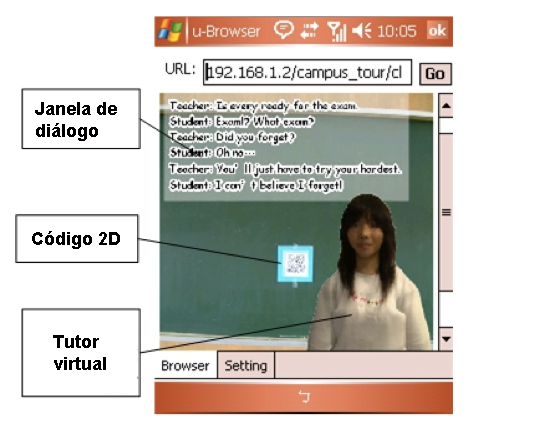
\includegraphics[scale=.7]{figuras/cap2/hello.png}
		\caption{\textit{Exemplo do tutor virtual utilizado no HELLO. Adaptado de~\cite{tsung}.}}
		\label{fig:hello} 
	\end{figure}